\documentclass{article}

\usepackage{geometry}
\usepackage{amsmath}
\usepackage{graphicx}
\usepackage{listings}
\usepackage{xcolor}
\usepackage{chngcntr}


\geometry{letterpaper, margin=1.5in, bottom=1in}

\counterwithin*{equation}{subsection}

\title{Problem Set Five}
\date{04/25/2018}
\author{Zhixian(Jason) Yu}

\definecolor{mygreen}{rgb}{0,0.6,0}
\definecolor{mygray}{rgb}{0.9,0.9,0.9}
\definecolor{mymauve}{rgb}{0.58,0,0.82}

\lstset{ %
  backgroundcolor=\color{mygray},   % choose the background color
  basicstyle=\footnotesize,        % size of fonts used for the code
  breaklines=true,                 % automatic line breaking only at whitespace
  captionpos=b,                    % sets the caption-position to bottom
  commentstyle=\color{mygreen},    % comment style
  escapeinside={\%*}{*)},          % if you want to add LaTeX within your code
  keywordstyle=\color{blue},       % keyword style
  stringstyle=\color{mymauve},     % string literal style
  keepspaces=true,
  tabsize=2,
  language=Python,
  numbersep=3pt, 
  numbers=left
  %frame=single
}

\begin{document}
\maketitle
\pagenumbering{gobble}
\newpage

\section{Theory}
\subsection*{Problem 3}
\paragraph{a)} Because $x$ is a single vector, we have:
\begin{align*}
\| x - \sum_{j \in N} w_j x_j \|^2 &= (x - \sum_{j \in N} w_j x_j)^T(x - \sum_{j \in N} w_j x_j) \\
&= (x^T - \sum_{j \in N} w_j x_j^T)(x - \sum_{j \in N} w_j x_j) \\
&= x^T x - \sum_{j \in N} w_j x^T x_j - \sum_{j \in N} w_j x_j^T x + \sum_{j \in N} w_j x_j^T\sum_{j \in N} w_j x_j \\
&= x^T x - \sum_{j \in N} w_j x^T x_j - \sum_{j \in N} w_j x_j^T x + \sum_{j \in N} w_j x_j^T\sum_{k \in N} w_k x_k \\
&= x^T x - \sum_{j \in N} w_j x^T x_j - \sum_{j \in N} w_j x_j^T x + \sum_{k \in N}\sum_{j \in N} w_j x_j^T (w_k x_k) \\
&= x^T x - \sum_{k \in N} w_k x^T x_k - \sum_{j \in N} w_j x_j^T x + \sum_{jk} w_j w_k x_j^T x_k
\end{align*}
Because $\sum_{j} w_j = 1$, we have $\sum_{k} w_k = 1$ and $\sum_{jk} w_j w_k = 1$. Therefore, the above equation becomes:
\begin{align*}
\| x - \sum_{j \in N} w_j x_j \|^2 &= x^T x - \sum_{k \in N} w_k x^T x_k - \sum_{j \in N} w_j x_j^T x + \sum_{jk} w_j w_k x_j^T x_k \\
&= \sum_{jk} w_j w_k x^T x - \sum_{j} w_j \sum_{k \in N} w_k x^T x_k - \sum_{k} w_k \sum_{j \in N} w_j x_j^T x + \sum_{jk} w_j w_k x_j^T x_k \\
&= \sum_{jk} w_j w_k x^T x - \sum_{jk} w_j w_k x^T x_k - \sum_{jk} w_j w_k x_j^T x + \sum_{jk} w_j w_k x_j^T x_k \\
&= \sum_{jk} w_j w_k (x^T x - x^T x_k - x_j^T x + x_j^T x_k) \\
&= \sum_{jk} w_j w_k (x-x_j)^T(x-x_k)
\end{align*}
Thus, \[ E(w) = \sum_{jk} w_j w_k C_{jk} \] where $C_{jk} = (x-x_j)^T(x-x_k)$.
\paragraph{b)}
Our goal is to minimize $\sum_{jk} w_j w_k C_{jk}$ subject to $\sum_{j} w_j = 1$. We can apply the method of Lagrange multipliers, and get:
\begin{align*}
L = \sum_{jk} w_j w_k C_{jk} - \lambda (\sum_{j} w_j - 1)
\end{align*}
If we take the partial derivative of $L$ over $w_j$, we get:
\begin{align*}
\frac{\partial L}{\partial w_j} &= 2w_jC_{jj} + \sum_{k \ne j} w_k C_{jk} + \sum_{k \ne j} w_k C_{kj} - \lambda \\
&= \sum_k w_k C_{jk} + \sum_k w_k C_{kj} - \lambda \\
&= 2 \sum_k w_k C_{jk} - \lambda
\end{align*}
Let $\frac{\partial L}{\partial w_j} = 0$, so:
\begin{align*}
\sum_k w_k C_{jk} = \frac{\lambda}{2}
\end{align*}
The above equation holds for any reasonable $j$, therefore:
\begin{align*}
w^T C = \frac{\lambda}{2} \vec{1}^{\,T}
\end{align*}
Because $C$ is a symmetric matrix, we can see that $w = C^{-T} \frac{\lambda}{2} \vec{1} = \frac{\lambda}{2} C^{-1} \vec{1}$. Expanding this leads to the following:
\begin{equation}
\label{eq: prob3b-1}
w_l = \frac{\lambda}{2} \sum_{m} C^{-1}_{lm}
\end{equation}
Because $\sum_{l} w_l = 1$, we have:
\begin{align*}
\sum_{l} w_l &= \sum_l \frac{\lambda}{2} \sum_{m} C^{-1}_{lm} \\
&= \frac{\lambda}{2} \sum_{lm} C^{-1}_{lm} \\
&= 1
\end{align*}
Therefore $\lambda = \frac{2}{\sum_{lm} C^{-1}_{lm}}$. Substitute the $\lambda$ from equation~\ref{eq: prob3b-1} with changes of some dummy indexes, we have:
\begin{align*}
w_j = \frac{\sum_{k} C^{-1}_{jk}}{\sum_{lm} C^{-1}_{lm}} 
\end{align*}

\paragraph{c)} Because $M = (I-W)^T(I-W)$, we have:
\begin{align*}
M_{ij} &= \sum_k (I-W)^T_{ik} (I-W)_{kj} \\
&= \sum_k (I^T_{ik} - W^T_{ik})(I_{kj} - W_{kj}) \\
&= \sum_k (I_{ik} - W_{ki})(I_{kj} - W_{kj}) \\
&= \sum_k I_{ik} I_{kj} - \sum_k I_{ik}W_{kj} - \sum_k W_{ki}I_{kj}  + \sum_k W_{ki} W_{kj} \\
&= \delta_{ij} - W_{ij} - W_{ji}  + \sum_k W_{ki} W_{kj} 
\end{align*}

\paragraph{d)} 
\begin{align*}
\sum_i {\| y_i - \sum_j W_{ij} y_j \|}^2 &= \sum_i (y_i - \sum_j W_{ij} y_j)^T (y_i - \sum_j W_{ij} y_j) \\
&= \sum_i (y_i^T - \sum_j W_{ij} y_j^T) (y_i - \sum_j W_{ij} y_j) \\
&= \sum_i y_i^T y_i - \sum_i y_i^T \sum_j W_{ij} y_j  - \sum_i \sum_j W_{ij} y_j^T y_i + \sum_i (\sum_j W_{ij} y_j^T \sum_j W_{ij} y_j) \\
&= \sum_i y_i^T y_i - \sum_i \sum_j W_{ij} y_i^T y_j  - \sum_i \sum_j W_{ij} y_j^T y_i + \sum_i \sum_k \sum_j W_{ik}y_k^T W_{ij} y_j 
\end{align*}
We can switch the indexes $i$ and $j$ in the term $\sum_i \sum_j W_{ij} y_j^T y_i$, switch the indexes $i$ and $k$ in the term $\sum_i \sum_k \sum_j W_{ik}y_k^T W_{ij} y_j$, and we get:
\begin{align*}
\sum_i {\| y_i - \sum_j W_{ij} y_j \|}^2 &= \sum_i \sum_j \delta_{ij} y_i^T y_j - \sum_i \sum_j W_{ij} y_i^T y_j  - \sum_j \sum_i W_{ji} y_i^T y_j + \sum_k \sum_i \sum_j W_{ki}y_i^T W_{kj} y_j \\
&= \sum_i \sum_j \delta_{ij} y_i^T y_j - \sum_i \sum_j W_{ij} y_i^T y_j  - \sum_i \sum_j W_{ji} y_i^T y_j + \sum_i \sum_j \sum_k W_{ki} W_{kj} y_i^T y_j \\
&= \sum_{i,j} (\delta_{ij} - W_{ij} - W_{ji} + \sum_k W_{ki}y_i^T W_{kj})y_i^T y_j \\
&= \sum_{i,j} M_{ij}y_i^T y_j
\end{align*}

\paragraph{e)}
\begin{align*}
trace(YMY^T) &= trace(MY^TY) \\
&= \sum_j \sum_i M_{ji} (Y^TY)_{ij} \\
&= \sum_i \sum_j M_{ji} y_i^T y_j
\end{align*}
Because $M^T = (I-W)^T(i-W) = M$, $M$ is a symmetric matrix, and $M_{ji} = M_{ij}$. Therefore:
\begin{align*}
trace(YMY^T) &= \sum_i \sum_j M_{ij} y_i^T y_j \\
&= \sum_i {\| y_i - \sum_j W_{ij} y_j \|}^2
\end{align*}

\paragraph{f)} We can use the Lagrangian multiplier method. So the optimization problem becomes

\newpage
\section{Programming}
The following code sets up the environment and import packages.
\begin{lstlisting}
	import numpy as np
	import matplotlib.pyplot as plt
	import matplotlib.image as mpimg
	import cv2
	import random
\end{lstlisting}

\subsection*{Problem 1}
%The following code reads image from file, and makes the color ranging from 0 to 1 instead of 0 to 255.  
%\begin{lstlisting}
%	img = mpimg.imread('./data/Penguins.jpg')
%	img = img/255
%\end{lstlisting}
%First thing is to randomly initialize 10 centers. The colors of the 10 random centers are shown in figure~\ref{fig:1_random_center}.
%\begin{lstlisting}
%	centers = [np.random.rand(3) for i in range(10)]  # randomly intialize 10 centers
%	for i in range(10):
%		plt.subplot(3,4,i+1)
%		plt.imshow(np.tile(centers[i], (10, 10, 1)))
%	plt.plot()
%\end{lstlisting}
%
%\begin{figure}[h!]
%\centering
%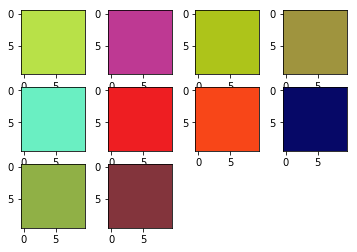
\includegraphics[width=0.6\linewidth]{../images/1_random_center.png}
%\caption{10 random colors that were initially picked.}
%\label{fig:1_random_center}
%\end{figure}
%
%The following code executes the LBG clustering algorithm. It was iterated 100 times. 
%\begin{lstlisting}
%	pixel_center_mapping = np.zeros((img.shape[0], img.shape[1])).astype(np.int8)
%	for i in range(100):
%		voronoi_set_sum = np.zeros((10,3))
%		voronoi_set_cnt = np.array([0 for i in range(10)])
%		for i in range(img.shape[0]):
%			for j in range(img.shape[1]):
%				distances = [np.linalg.norm(centers[k] - img[i][j]) for k in range(10)]
%				closest_ind = np.argmin(distances)
%				pixel_center_mapping[i][j] = closest_ind
%				voronoi_set_sum[closest_ind] += img[i][j]
%				voronoi_set_cnt[closest_ind] += 1
%		for i in range(10):
%			if voronoi_set_cnt[i] != 0:
%				centers[i] = voronoi_set_sum[i]/voronoi_set_cnt[i]
%\end{lstlisting}
%After clustering, the center colors are shown in figure~\ref{fig:1_trained_center}.
%\begin{lstlisting}
%	for i in range(10):
%		plt.subplot(3,4,i+1)
%		plt.imshow(np.tile(centers[i], (10, 10, 1)))
%	plt.plot()
%\end{lstlisting}
%
%\begin{figure}[h!]
%\centering
%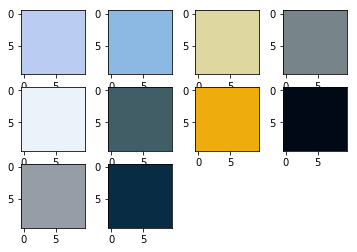
\includegraphics[width=0.6\linewidth]{../images/1_trained_center.png}
%\caption{10 center colors after LBG clustering.}
%\label{fig:1_trained_center}
%\end{figure}
%
%The following code is used to produce the color-quantized new picture, which is shown in figure~\ref{fig:1_new_penguin}. As is shown, the sky was approximately quantized to 3 regions, and the penguins are quantized to about 4-5 colors. 
%\begin{lstlisting}
%	new_img = np.copy(img)
%	for i in range(img.shape[0]):
%		for j in range(img.shape[1]):
%			new_img[i][j] = centers[pixel_center_mapping[i][j]]
%	plt.imshow(new_img)
%	plt.show()
%\end{lstlisting}
%
%\begin{figure}[h!]
%\centering
%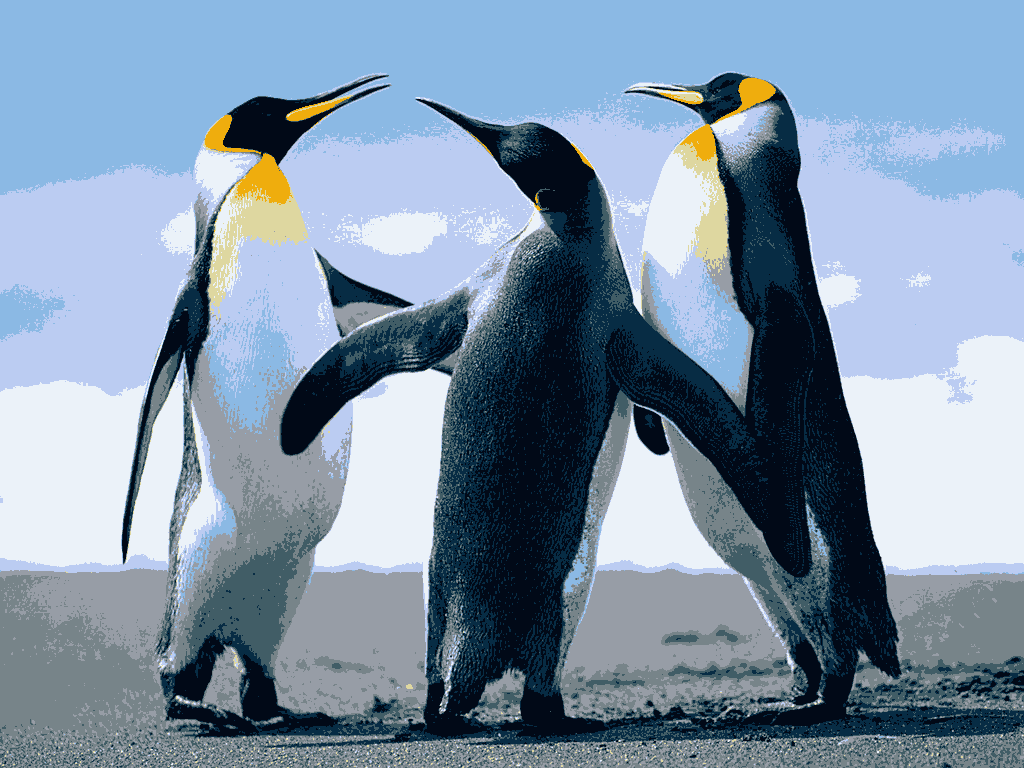
\includegraphics[width=0.6\linewidth]{../images/1_new_penguin.png}
%\caption{Color quantized image.}
%\label{fig:1_new_penguin}
%\end{figure}

\end{document}
